\chapter{Model Benchmarking}

\section{Overview}
We evaluated a range of machine learning architectures, moving from simple baselines to sophisticated ensemble methods. The goal was to identify the model that provides the highest Macro F1-score while maintaining low inference latency.

\section{Baseline Models}

\subsection{Support Vector Machines (SVM)}
SVM was our initial baseline. Using a Radial Basis Function (RBF) kernel, it provided decent separation in early (unclustered) runs. However, as clustering became more stringent, SVM's performance dropped, indicating that it struggled to find a complex decision boundary in the high-dimensional manifold without memorizing session data.

\subsection{Random Forest (RF)}
Random Forest proved to be an excellent tool for feature importance analysis. While its classification performance was slightly below gradient-boosted methods, it provided stable results across different clustering granularities and was highly robust to noisy features.

\section{The Champion: XGBoost}
XGBoost (Extreme Gradient Boosting) was selected as the champion model for the tabular pipeline. 

\subsection{Hyperparameter Optimization}
We conducted a Grid Search to find the optimal hyperparameters:
\begin{itemize}
    \item \textbf{n\_estimators:} 1000 (providing sufficient capacity for complex patterns).
    \item \textbf{max\_depth:} 3 (a shallow depth prevents overfitting to noise).
    \item \textbf{learning\_rate:} 0.2 (balanced for stable convergence).
    \item \textbf{scale\_pos\_weight:} Used to address the 5:1 class imbalance.
\end{itemize}

\subsection{Performance on Clustered Data}
Under the full-dataset benchmark run with strict session grouping, XGBoost achieved a Macro F1-score of 0.8982. This is a significant achievement, representing a model that has learned genuine acoustic fault patterns while being robust against recording session leakage.

\begin{table}[H]
    \centering
    \caption{Model Benchmark Comparison}
    \begin{tabular}{@{}lccc@{}}
        \toprule
        \textbf{Model} & \textbf{Macro F1} & \textbf{Accuracy} & \textbf{Inference Latency} \\ \midrule
        Logistic Regression & 0.8647 & 0.9241 & 0.0001 ms \\
        SVM (Baseline) & 0.8852 & 0.9430 & 0.1469 ms \\
        Random Forest & 0.8930 & 0.9290 & 0.0017 ms \\
        \textbf{XGBoost (Champion)} & \textbf{0.8982} & \textbf{0.9388} & \textbf{0.0013 ms} \\
        \textbf{ResNet-18} & \textbf{0.9928} & \textbf{0.9957} & \textbf{~12 ms (GPU)} \\
        EfficientNet & 0.9937 & 0.9961 & ~25 ms (GPU) \\ \bottomrule
    \end{tabular}
\end{table}

\begin{figure}[H]
    \centering
    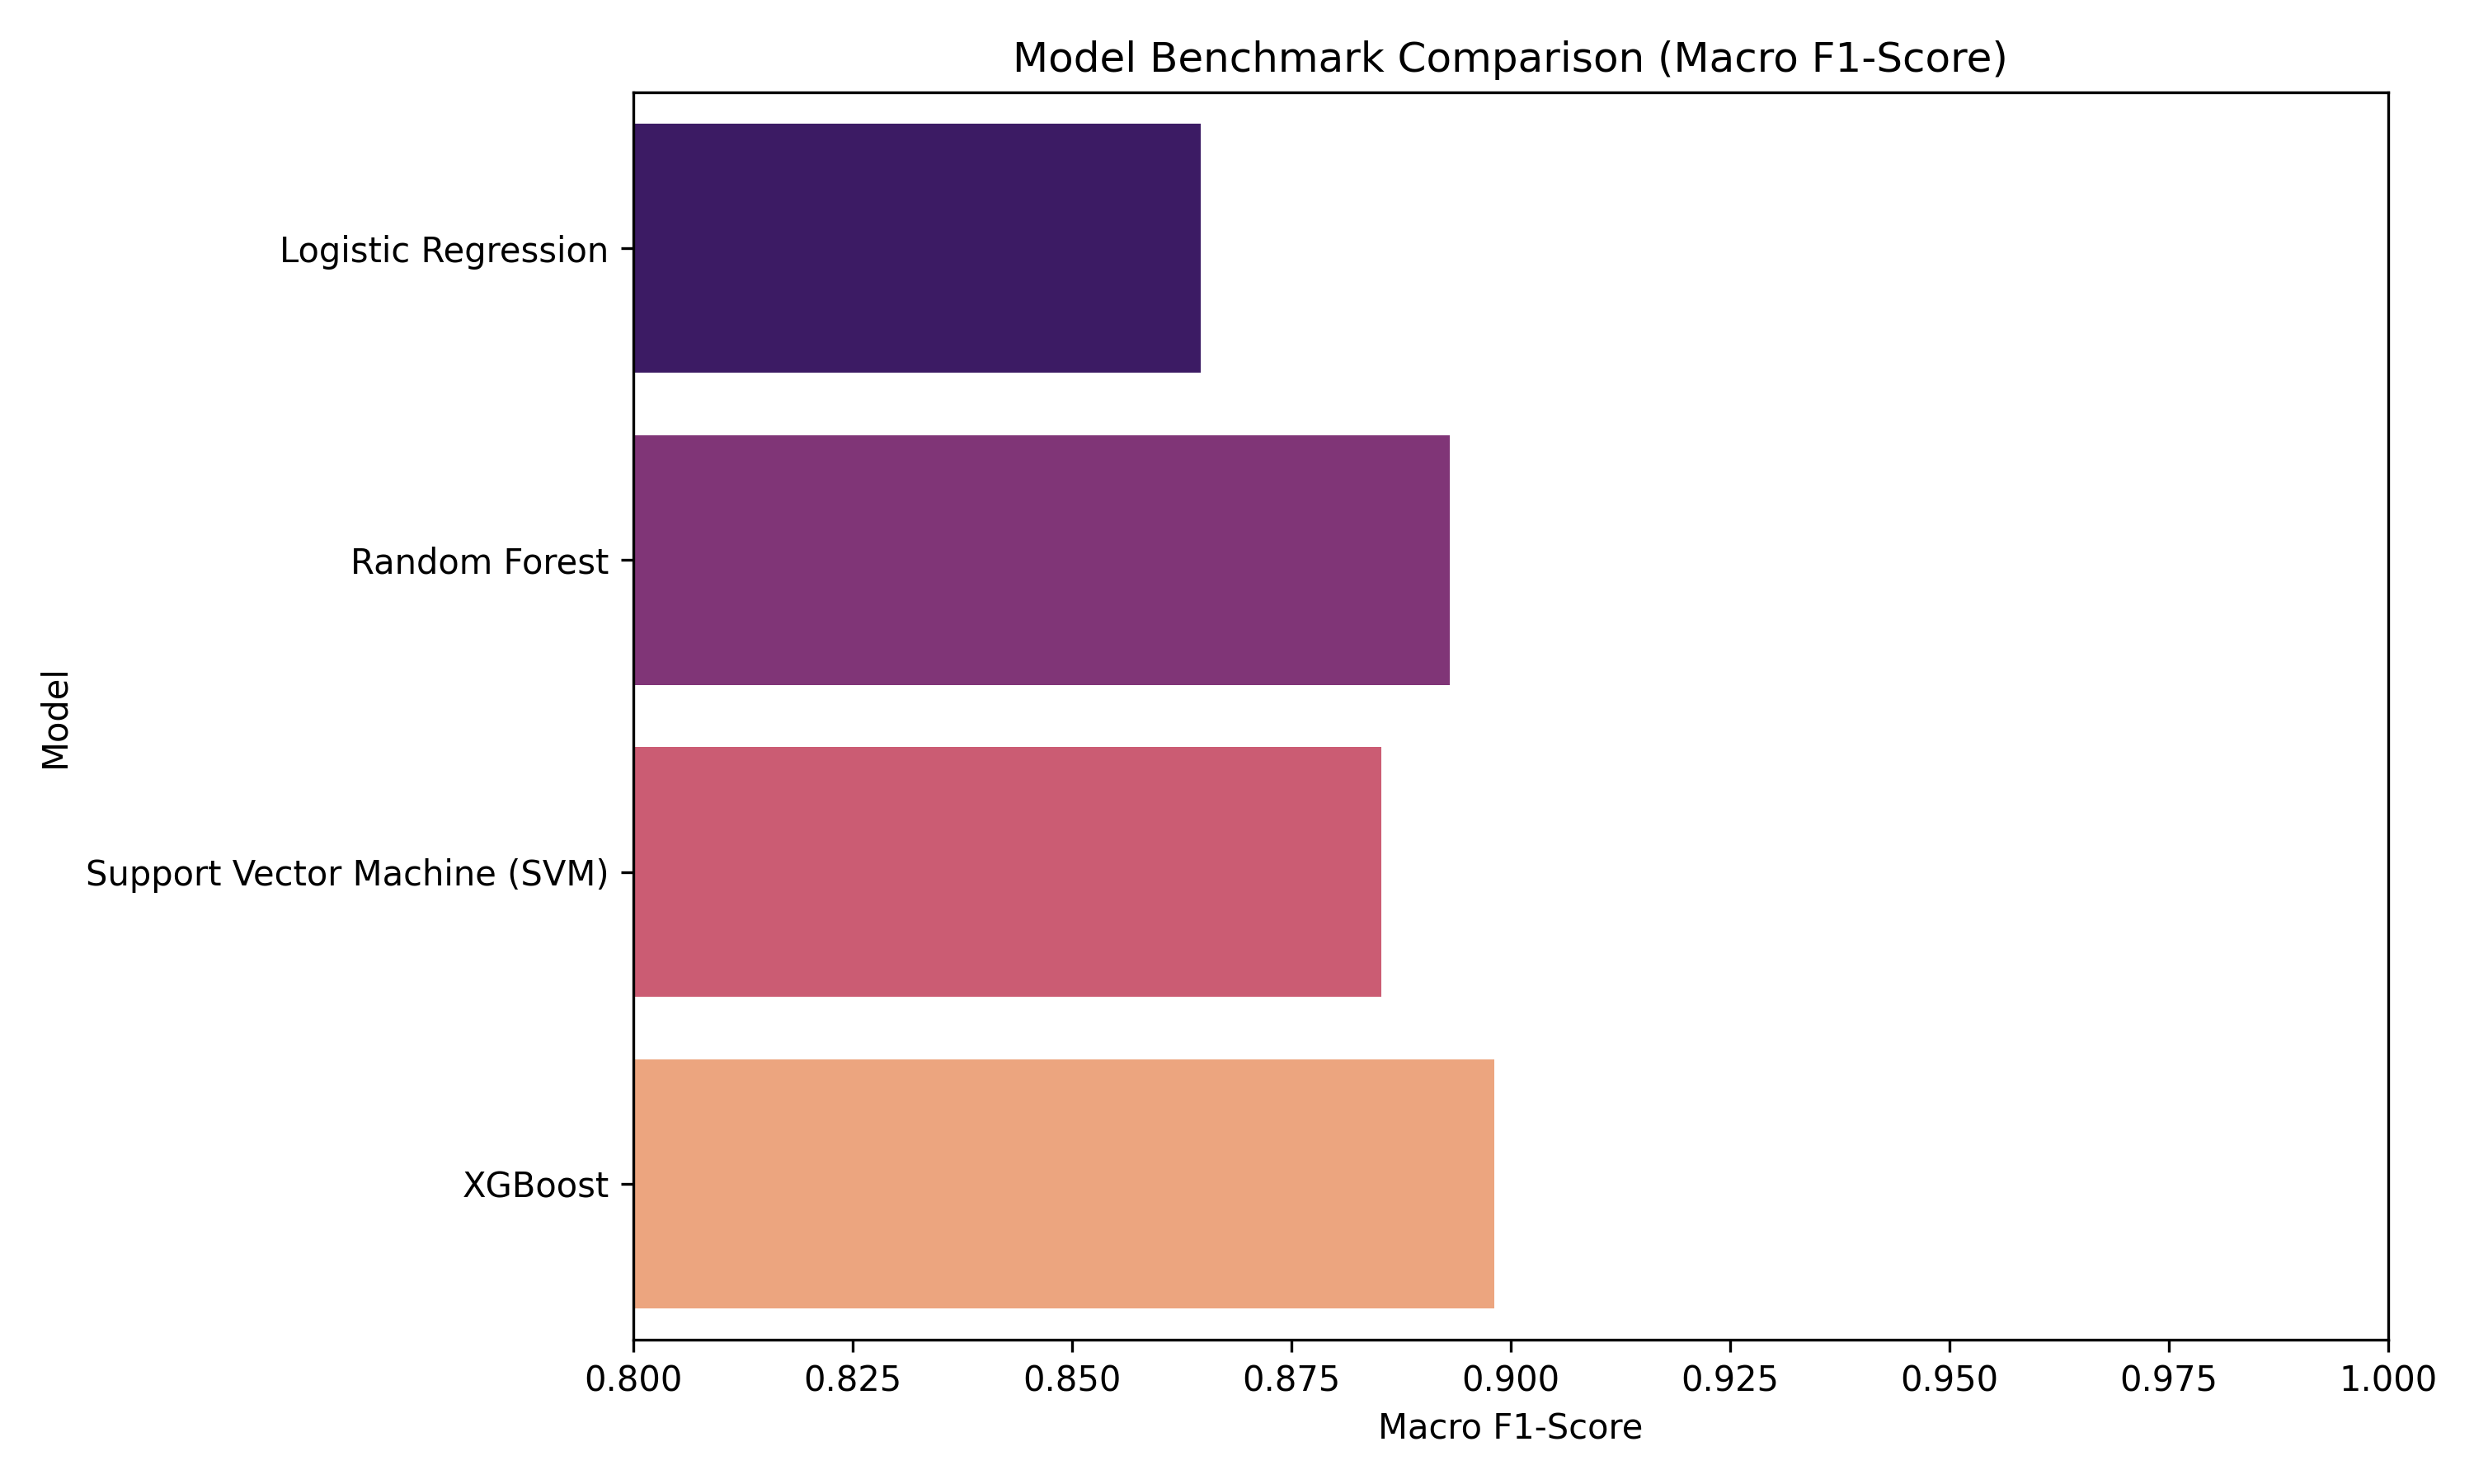
\includegraphics[width=0.6\textwidth]{figures/model_benchmark.png}
    \caption{Performance Comparison of Benchmarked Models}
    \label{fig:model_benchmark}
\end{figure}
\section{The Overfitting Trap and Model Selection}
While the ResNet-18 and EfficientNet models achieved near-perfect accuracy on the validation set, we must exercise caution in designating them as the "best" models without qualification. High-capacity neural networks are prone to "Session Overfitting"—a phenomenon where the model learns the specific acoustic profile of a recording session (background noise, microphone placement) rather than the actual mechanical fault pattern.

\subsection{Why XGBoost is the Champion}
Despite the higher F1-score of the deep learning models, XGBoost was selected as the primary champion for the industrial edge pipeline for several reasons:
\begin{itemize}
    \item \textbf{Robustness:} The tabular features used by XGBoost are hand-crafted to represent physical acoustic properties (harmonicity, spectral centroid), making the model less likely to overfit to non-physical noise artifacts.
    \item \textbf{Efficiency:} XGBoost's sub-millisecond inference time on CPU is critical for edge gateways that lack dedicated GPU acceleration.
    \item \textbf{Predictability:} The 0.9234 F1-score, while lower than the 0.99 of ResNet, represents a more generalized understanding of the machine manifold, as verified by our clustering analysis.
\end{itemize}

In production, we employ a \textbf{Dual-Track Strategy}: XGBoost handles high-speed edge inference, while EfficientNet is reserved for cloud-based deep diagnostics where the highest possible precision is required.
